% ../../../1994_全国卷_理科/figures/f1994_national_science_q12_inverse_graphs.tex — 1994 年·全国卷·理科 第 12 题（四图象选项）
%
% 【来源】`.work/phase4-b19/source/1994全国理.pdf`（SHA-256 e4511d861907c36870489c60d5f150690c8d7d5c10805937609a3bb62c532a2f），第 1 页；
%   内容流逐路径照录，本地坐标 = 页面坐标 − (458.700,612.000)，1 单位 = 1 TeX pt。
%   每个 m 子路径独立起笔；线宽/虚线按内容流原值；标签取 pdftotext -bbox 中心。
%
% 元素计数：24 路径＋24 标签
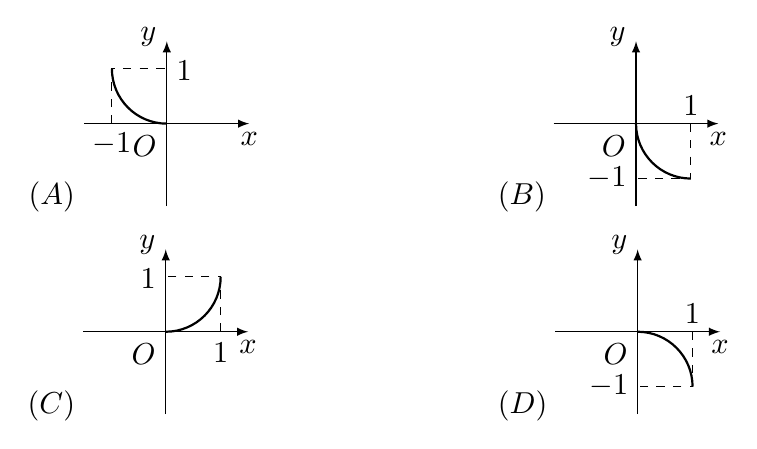
\begin{tikzpicture}[x=1pt, y=1pt,
    every node/.style={inner sep=0pt, font=\fontsize{10.5pt}{12.6pt}\selectfont}]
  \draw[line width=0.398pt] (0.378,104.792) -- (56.319,104.792);
  \fill[line width=1.0pt] (59.906,104.792) .. controls (58.843,104.991) and (57.116,105.589) .. (55.921,106.286) -- (55.921,103.298) .. controls (57.116,103.995) and (58.843,104.593) .. (59.906,104.792);
  \draw[line width=0.398pt] (30.142,75.028) -- (30.142,130.969);
  \fill[line width=1.0pt] (30.142,134.556) .. controls (29.943,133.493) and (29.345,131.766) .. (28.648,130.571) -- (31.636,130.571) .. controls (30.939,131.766) and (30.341,133.493) .. (30.142,134.556);
  \draw[line width=0.398pt, dash pattern=on 2.989pt off 2.989pt] (10.299,104.792) -- (10.299,124.635) -- (30.142,124.635);
  \draw[line width=0.797pt] (30.142,104.792) .. controls (19.183,104.792) and (10.299,113.676) .. (10.299,124.635);
  \draw[line width=0.398pt] (169.928,104.792) -- (225.869,104.792);
  \fill[line width=1.0pt] (229.456,104.792) .. controls (228.393,104.991) and (226.666,105.589) .. (225.471,106.286) -- (225.471,103.298) .. controls (226.666,103.995) and (228.393,104.593) .. (229.456,104.792);
  \draw[line width=0.398pt] (199.692,75.028) -- (199.692,130.969);
  \fill[line width=1.0pt] (199.692,134.556) .. controls (199.493,133.493) and (198.895,131.766) .. (198.198,130.571) -- (201.186,130.571) .. controls (200.489,131.766) and (199.891,133.493) .. (199.692,134.556);
  \draw[line width=0.398pt, dash pattern=on 2.989pt off 2.989pt] (219.535,104.792) -- (219.535,84.949) -- (199.692,84.949);
  \draw[line width=0.797pt] (199.692,104.792) .. controls (199.692,93.833) and (208.576,84.949) .. (219.535,84.949);
  \draw[line width=0.398pt] (-0.004,29.596) -- (55.937,29.596);
  \fill[line width=1.0pt] (59.524,29.596) .. controls (58.461,29.795) and (56.734,30.393) .. (55.539,31.090) -- (55.539,28.102) .. controls (56.734,28.799) and (58.461,29.397) .. (59.524,29.596);
  \draw[line width=0.398pt] (29.760,-0.168) -- (29.760,55.773);
  \fill[line width=1.0pt] (29.760,59.360) .. controls (29.561,58.297) and (28.963,56.570) .. (28.266,55.375) -- (31.254,55.375) .. controls (30.557,56.570) and (29.959,58.297) .. (29.760,59.360);
  \draw[line width=0.398pt, dash pattern=on 2.989pt off 2.989pt] (49.603,29.596) -- (49.603,49.439) -- (29.760,49.439);
  \draw[line width=0.797pt] (29.760,29.596) .. controls (40.719,29.596) and (49.603,38.480) .. (49.603,49.439);
  \draw[line width=0.398pt] (170.516,29.596) -- (226.457,29.596);
  \fill[line width=1.0pt] (230.044,29.596) .. controls (228.981,29.795) and (227.254,30.393) .. (226.059,31.090) -- (226.059,28.102) .. controls (227.254,28.799) and (228.981,29.397) .. (230.044,29.596);
  \draw[line width=0.398pt] (200.280,-0.168) -- (200.280,55.773);
  \fill[line width=1.0pt] (200.280,59.360) .. controls (200.081,58.297) and (199.483,56.570) .. (198.786,55.375) -- (201.774,55.375) .. controls (201.077,56.570) and (200.479,58.297) .. (200.280,59.360);
  \draw[line width=0.398pt, dash pattern=on 2.989pt off 2.989pt] (220.123,29.596) -- (220.123,9.753) -- (200.280,9.753);
  \draw[line width=0.797pt] (200.280,29.596) .. controls (211.239,29.596) and (220.123,20.712) .. (220.123,9.753);
  \node[anchor=center] at (23.490,136.050) {$y$};
  \node[anchor=center] at (59.910,99.310) {$x$};
  \node[anchor=center] at (22.150,96.650) {$O$};
  \node[anchor=center] at (36.470,123.990) {$1$};
  \node[anchor=center] at (10.300,97.590) {$-1$};
  \node[anchor=center] at (-11.430,78.150) {$(A)$};
  \node[anchor=center] at (193.040,136.050) {$y$};
  \node[anchor=center] at (229.460,99.310) {$x$};
  \node[anchor=center] at (191.700,96.650) {$O$};
  \node[anchor=center] at (219.540,111.230) {$1$};
  \node[anchor=center] at (189.280,85.260) {$-1$};
  \node[anchor=center] at (158.430,78.150) {$(B)$};
  \node[anchor=center] at (23.110,60.860) {$y$};
  \node[anchor=center] at (59.520,24.110) {$x$};
  \node[anchor=center] at (21.760,21.460) {$O$};
  \node[anchor=center] at (23.440,48.790) {$1$};
  \node[anchor=center] at (49.600,21.870) {$1$};
  \node[anchor=center] at (-11.570,2.960) {$(C)$};
  \node[anchor=center] at (193.630,60.860) {$y$};
  \node[anchor=center] at (230.040,24.110) {$x$};
  \node[anchor=center] at (192.280,21.460) {$O$};
  \node[anchor=center] at (220.120,36.030) {$1$};
  \node[anchor=center] at (189.870,10.070) {$-1$};
  \node[anchor=center] at (158.730,2.960) {$(D)$};
\end{tikzpicture}
%
% 【自验结果】逐路径照录；探针编译 0 警告。
